\documentclass{report}
\usepackage{graphicx}
\usepackage{float}
\usepackage[a4paper, top=20mm, bottom=20mm, left=25mm, right=25mm]{geometry}
\usepackage{subcaption}
\usepackage{titlesec}
\title{Visual Computing Assignment 4}

\author{Ebbe Wertz, Mathias Houwen}
\date{22 April 2025}

\begin{document}

\maketitle

\section{Modelling}

Every item was modeled using 3D cube objects with adjusted scaling. These were all given a mesh renderer with a custom material. Every object additionally also has a box collider to make sure that blocks will collide with any side of the bins. \\
To model the blocks, the same method was used, but the object was then then moved to the project folder and deleted from the scene. This way, the block could be kept as a reusable prefab object. Additionally, a rigidBody was also added to the object in order to fall by gravity.\\

\section{Block spawning}

To spawn in blocks, a script was made and attached to an empty game object acting as the spawn point. When spawning, it first uses the transform property of this object to determine the spawning location. A \textit{Vector3} with small randomised dimensions is added to this location as an offset in order to provide slight randomisation in space. It then uses the \textit{Instantiate} function to generate an instance of the block prefab into the scene. After this, the parent propery of the block is set to the transform propery of the pickup bin. Figure \ref{fig:30spawn} shows the model of the bins and robots, where 30 blocks were spawned in the pickup bin.

\begin{figure}[H]
\centering
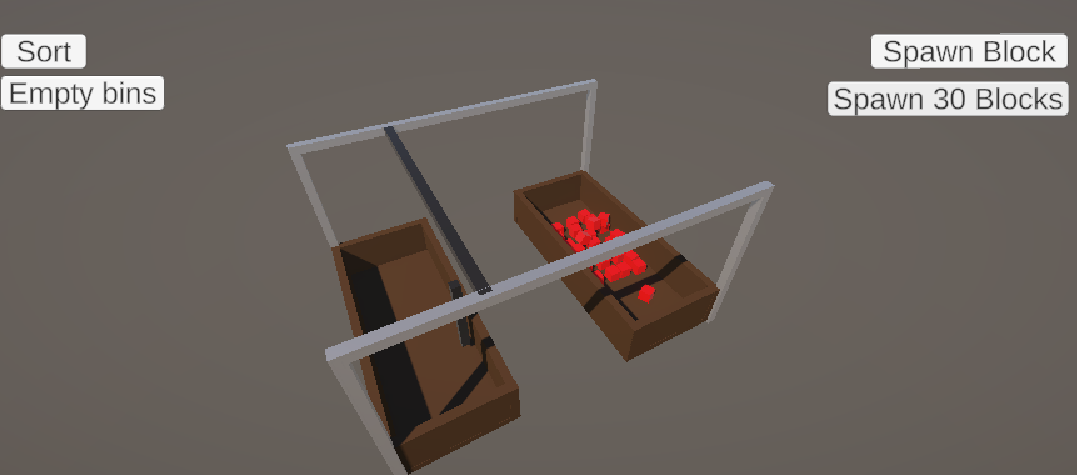
\includegraphics[height=50mm, keepaspectratio]{report_images/30spawn.png}
\caption{Bin model containing 30 block objects.}
\label{fig:30spawn}
\end{figure}

\section{Block detection}

In order for the robot to pick up blocks, they need to be detected in the pickup bin. Newly spawned blocks are already assigned to the pickup bin as their parent, but to use a more realistic approach, another detection mechanism is added.
Firstly, a script is created that can be attached to any game object representing a bin (which groups the cubes, composing the bin shape).
This game object is also given an additional box collider that spans the full bounding box of the bin. This box collider will be used in the script to detect if blocks are inside the bin. To prevent physical collisions, the \textit{Is Trigger} property is checked. This disables any physics and will make the box collider only a detector. Since the cubes composing the bin itself are also colliding with this, they should be ignored. This is done by defining a unique block tag in unity which is then assigned to the block prefab object. By checking if the tag equals "block", any non-block objects in the collision area are ignored. By this logic the script could expose a function returning a list of game objects which are the detected blocks inside a bin. This function will be used to clear bins as well as for the robot to pick up blocks. Figure \ref{fig:coll} shows in green outline both the collision areas of the individually composing cubes as well as the bigger encapsulating one used for detection.

\begin{figure}[H]
\centering
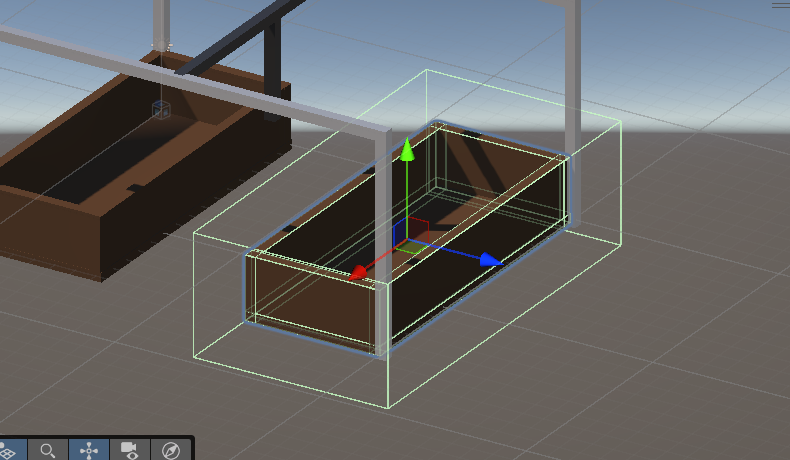
\includegraphics[height=50mm, keepaspectratio]{report_images/coll.png}
\caption{Collision areas of a bin.}
\label{fig:coll}
\end{figure}

\section{Robot}
To control the robot arm there are two main components: a horizontal beam and a vertical beam. The goal is to move the tip of the robot arm smoothly to a target 3D position in a safe and controlled sequence. The \textit{Robot.cs} script acts as the controller.  It references the horizontal and vertical beams and listens for user input. \\ % interfaceing with the cubs
The actual movement logic is handled by the \textit{RobotMovement.cs} script, which is attached to the same GameObject as the \textit{Robot.cs} script. At the core of movement logic is a finite state machine (FSM). In this case, the FSM has the flowing states:
\begin{itemize}
    \item \textbf{None}: Idle, waiting for a new command
    \item \textbf{MoveUP}: The robot lifts the tip vertically to clear the workspace.
    \item \textbf{MoveZ}: The robot moves along the Z-axis.
    \item \textbf{MoveX}: The robot moves along the X-axis.
    \item \textbf{MoveDown}: The robot lowers the tip to the final Y-position
\end{itemize}
The transition between these states occurs sequentially and is controlled by conditions based on the current tip position and the desired target. Each state performs a small part of the total movement, ensuring that the robot moves safely and predictably. The order of these states are shown in figure~\ref{fig:FSM}.

\begin{figure}[H]
\centering
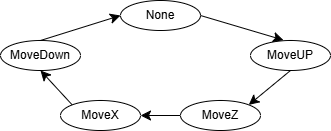
\includegraphics[height=50mm, keepaspectratio]{report_images/diagram.drawio.png}
\caption{Finite state machine.}
\label{fig:FSM}
\end{figure}

\section{ Block transfer}
For the full block transfer process, an additional state machine was added to the robot, on a higher level, including a \textit{PickingUP} and \textit{DroppingOff} state.
When the robot is assigned to transfer a block to a location, first the state is set to \textit{PickingUP}. Then instance variables of the script class hold the game object reference to the block, the transform reference to the parent bin, the target position, and a placeholder for a callback function.\\
In the transfer process, first it will extract the block location from its transform propery and use the low level state machine to move the robot to that location. When arrived, the block's parent property is transferred to the vertical beam component of the robot. Additionally, the \textit{isKinematic} property of the block's rigidBody is set to \textit{true} and the \textit{useGravity} to \textit{false}. This disables gravity and allows the block to move along with its parent, now being the robot's vertical beam. Both these properties are encapsulated into a function \textit{makeBlockStick(GameObject block, bool stick)} in order to easily reverse the effect later.\\
\newline
Now that the robot arrived to the block's location and the block is attached to the robot arm, the high level state is switched to the \textit{DroppingOff} state. The robot now uses the low level state machine to move to the target location saved in the instance variable. When arriving, it tranfers the block's parent property to the target transform, which is via the unity editor assigned to the drop off bin. Then it uses the \textit{makeBlockStick} function to re-enable gravity, allowing the block to release.

\section{Top level control loop}

In order to repeat the block transfer process, a controller script was made, attached to an empty game object. This script uses the block detection script attached to the pickup bin to fetch a list of all blocks to be transferred. Using an IEnumerator, it constructs an asynchronous loop that can repeatedly call the robot's block transfer function, while it passes a simple lambda function as the callback function. This lambda toggles a flag variable. \textit{WaitUntil} is used to block the loop during transfer.

\section{Block positioning}

In order to align blocks in a grid shape, the controller uses a function to first calculate the target location before passing it to the robot's transfer function. In order to define the gird, first a plane object is added inside the drop off bin. This plane is not assigned a material and the mesh renderer is disabled as this plane is only used to define the dimensions of the grid.
Figure \ref{fig:plane} shows this plane with the mesh renderer temporarily turned on.

\begin{figure}[H]
\centering
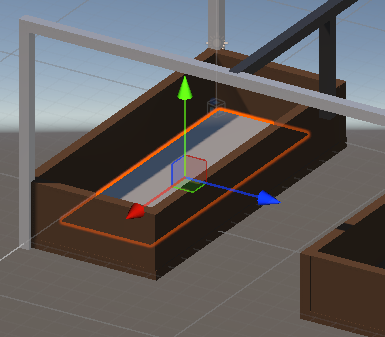
\includegraphics[height=50mm, keepaspectratio]{report_images/plane.png}
\caption{Grid bounding plane.}
\label{fig:plane}
\end{figure}

The dimensions of this plane object and a field for the number of rows and columns are then used to calculate a position in the grid based on an index. (this index is a number incremented from zero). This index simply corresponds to the iteration index of the main control loop. To handle a case of overflow, the grid positions are always clipped to stay within the specified dimensions. When the grid is filled, the y coordinate is increased, stacking the grid further vertically.\\
\newline
Figure \ref{fig:sort} finally shows the robot in action, transferring blocks from the pickup bin to aligned positions in the drop off bin.
\begin{figure}[H]
\centering
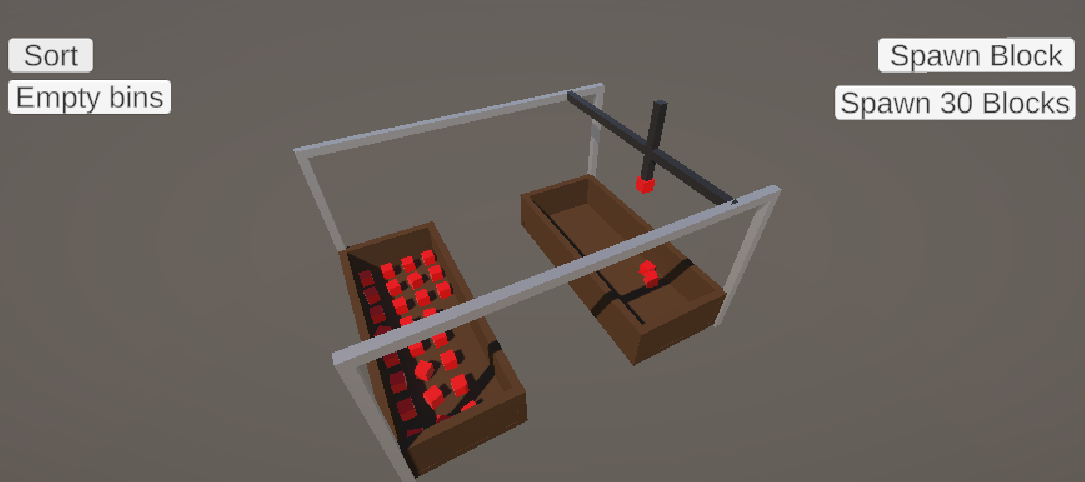
\includegraphics[height=50mm, keepaspectratio]{report_images/sorting.png}
\caption{Robot transferring blocks}
\label{fig:sort}
\end{figure}

\end{document}